%% !TEX root = manual.tex

\section{Fat Tree}
\label{sec:tutorial:fattree}

Within SST, a fat tree is defined by the following parameters:

\begin{ViFile}
topology.name = fattree
topology.geometry = 4 2
\end{ViFile}
The first number, 4, indicates the number of levels in the fat tree.
The second number, 2, indicates the radix or branching factor of the tree.
The number of compute nodes in this topology is $2^4 = 16$.
This is illustrated conceptually in Figure \ref{fig:topologies:abstractfattree}.
The color coding will become clear later.
We note this is somewhat confusing since the fat tree appears to have 5 levels.
Here the topology is defined by the number of levels containing switches or the number of branches.
This is done for a very specific reason.  
At the final level, you may wish to have a different branching fraction for the compute nodes, e.g.

\begin{ViFile}
topology.concentration = 1
\end{ViFile}
This loads the injection bandwidth for the compute node dedicating its own injection switch.
If the parameter \inlineshell{network_nodes_per_switch} is omitted, it defaults to the fat tree radix.
This case is shown in Figure \ref{fig:topologies:abstractfattree} where there are two nodes injecting to the same switch.
Higher radix fat trees can be specified, e.g.

\begin{ViFile}
topology.name = fattree
topology.geometry = 3 4
\end{ViFile}
which would have $4^3 = 64$ compute nodes.

\begin{figure}[h!]
\centering
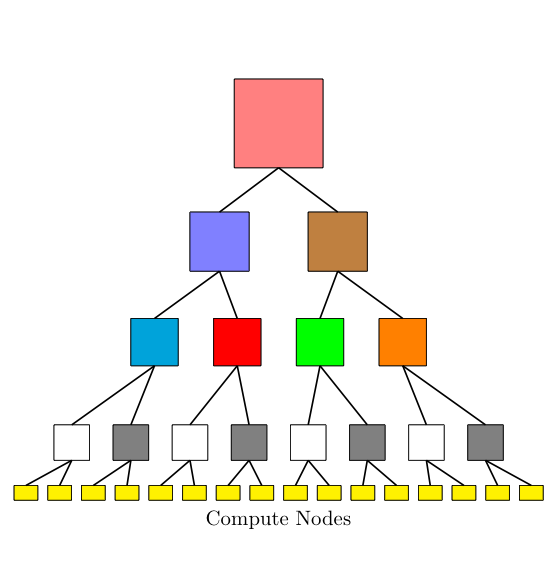
\includegraphics[width=0.9\textwidth]{figures/tikz/fattree/abstract_fattree.png}
\caption{Abstract, conceptual picture of Fat Tree topology}
\label{fig:topologies:abstractfattree}
\end{figure}

In reality, it is not practical to implement a fat tree exactly as shown in Figure \ref{fig:topologies:abstractfattree}.
One would need to buy many non-standard, high capacity switches for the higher levels in the fat-tree.
The simple model is available by specifying \inlineshell{simple_fattree} as the topology, and SST will construct special large switches at higher levels.
The best practical implementation employs all uniform, commodity switches (Figure \ref{fig:topologies:fattreeids}).
The fat tree is ``virtual'' with several commodity switches grouped together to simulate a heavy-weight, high capacity switch
at higher levels of the fat tree.
The connection between the physical implementation and the conceptual fat tree can easily be seen by the color coding.
For example, the second row contains eight switches, but only two virtual switches.
Each virtual switch is composed of four commodity switches.

\begin{figure}[h!]
\centering
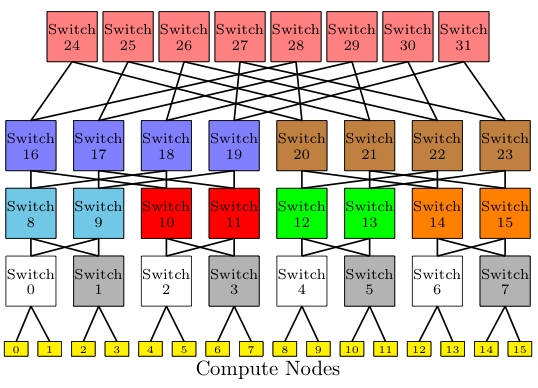
\includegraphics[width=0.9\textwidth]{figures/tikz/fattree/fattree_ids.png}
\caption{Physical implementation of Fat Tree with commodity switches showing ID numbering}
\label{fig:topologies:fattreeids}
\end{figure}

Within SST, each switch is assigned a unique ID, starting from zero in the bottom row and proceeding through the top level.
In addition, each compute node is also assigned a unique ID from 0 to 15.
The switches can also be defined by a set of coordinates.
While the choice of coordinate system for a 3D torus is obvious, 
the coordinate system for the fat tree is less clear.
In SST, we define a 2D mesh coordinate system for the row (level) and column of the switch.


\subsection{Allocation and indexing}
\label{subsec:fattree:allocation}
The numbering of compute nodes is shown in Figure \ref{fig:topologies:fattreeids}.
Consider the case

\begin{ViFile}
app1.launch_cmd = aprun -n 4 -N 1
\end{ViFile}
which launches four processes all on distinct nodes.
In the simplest allocation and indexing scheme (first available),
processes would be placed in order on 0,1,2,3.
An alternative allocation/indexing scheme uses the Node ID allocator.

\begin{ViFile}
app1.allocation = node_id
app1.indexing = node_id
app1.node_id_file = nodes.txt
\end{ViFile}
Here \inlineshell{nodes.txt} would contain the number of nodes on the first line, followed by the list of Node IDs, in order, of where to place MPI ranks.
For the file

\begin{ViFile}
4
0
4
8
12
\end{ViFile}
Four MPI ranks would be placed in spatially distant parts of the machine.

If indexing differs from allocation (usually because there are multiple MPI ranks per node), both an allocation and an indexing file are needed.
Suppose we have:

\begin{ViFile}
app1.launch_cmd = aprun -n 4 -N 2
\end{ViFile}
We then need:

\begin{ViFile}
app1.allocation = node_id
app1.indexing = node_id
app1.node_id_allocation_file = alloc.txt
app1.node_id_indexing_file = index.txt
\end{ViFile}
where the contents of \inlineshell{alloc.txt} are, e.g.

\begin{ViFile}
2
0
1
\end{ViFile}
choosing nodes 0 and 1 in the allocation and then \inlineshell{index.txt} would be, e.g.

\begin{ViFile}
4
0
1
0
1
\end{ViFile}
which round-robin assigns rank 0 to node, rank 1 to node 1, rank 2 to node 0, and so on.

\subsection{Routing}
\label{subsec:fattree:routing}

Fat tree routing is actually straightforward, but can employ path diversity.
Suppose you are routing from Node 0 to Node 2 (Figure \ref{fig:topologies:fattreeids}).
At the first stage, you have no choice.
You must route to Switch 1.
At the second stage, you can either route to Switch 8 or Switch 9.
Suppose you branch to Switch 9. 
At this point, you are done moving up.
The packet now proceeds down the fat-tree.
On the downward routing, there is no path diversity.
Only a single, minimal route exists to the destination node.
In the simplest case, Switch 1 alternates between selecting Switch 8 and Switch 9 to distribute load.
In a more complicated scheme, Switch 1 could adaptively route selecting either Switch 8 or Switch 9 based on congestion information.
